\section{Parser}

Das Ziel des Parsers ist es, den Programmcode in eine Struktur zu bringen, die vom Interpreter interpretiert werden kann. Beim Lesen eines Programmcodes, wird dieser auch auf syntaktische Korrektheit überprüft. Dies geschieht mithilfe einer gegebenen Syntax in der Sprachbeschreibung.
Das Parsen wird in diesem Projekt in zwei Schritten umgesetzt. Im Unterkapitel \ref{subsection:parser} wird die Umwandlung des Programmcodes in eine Parserstruktur beschrieben. In Unterkapitel \ref{subsection:ast} wird diese dann in eine Baumstruktur gebracht, die dann an den Interpreter weiter gegeben wird. 

\subsection{Ziel}

\begin{figure}[tbh]
	%\centering
	%\hspace{-0.1\linewidth}
	%\fbox{}
	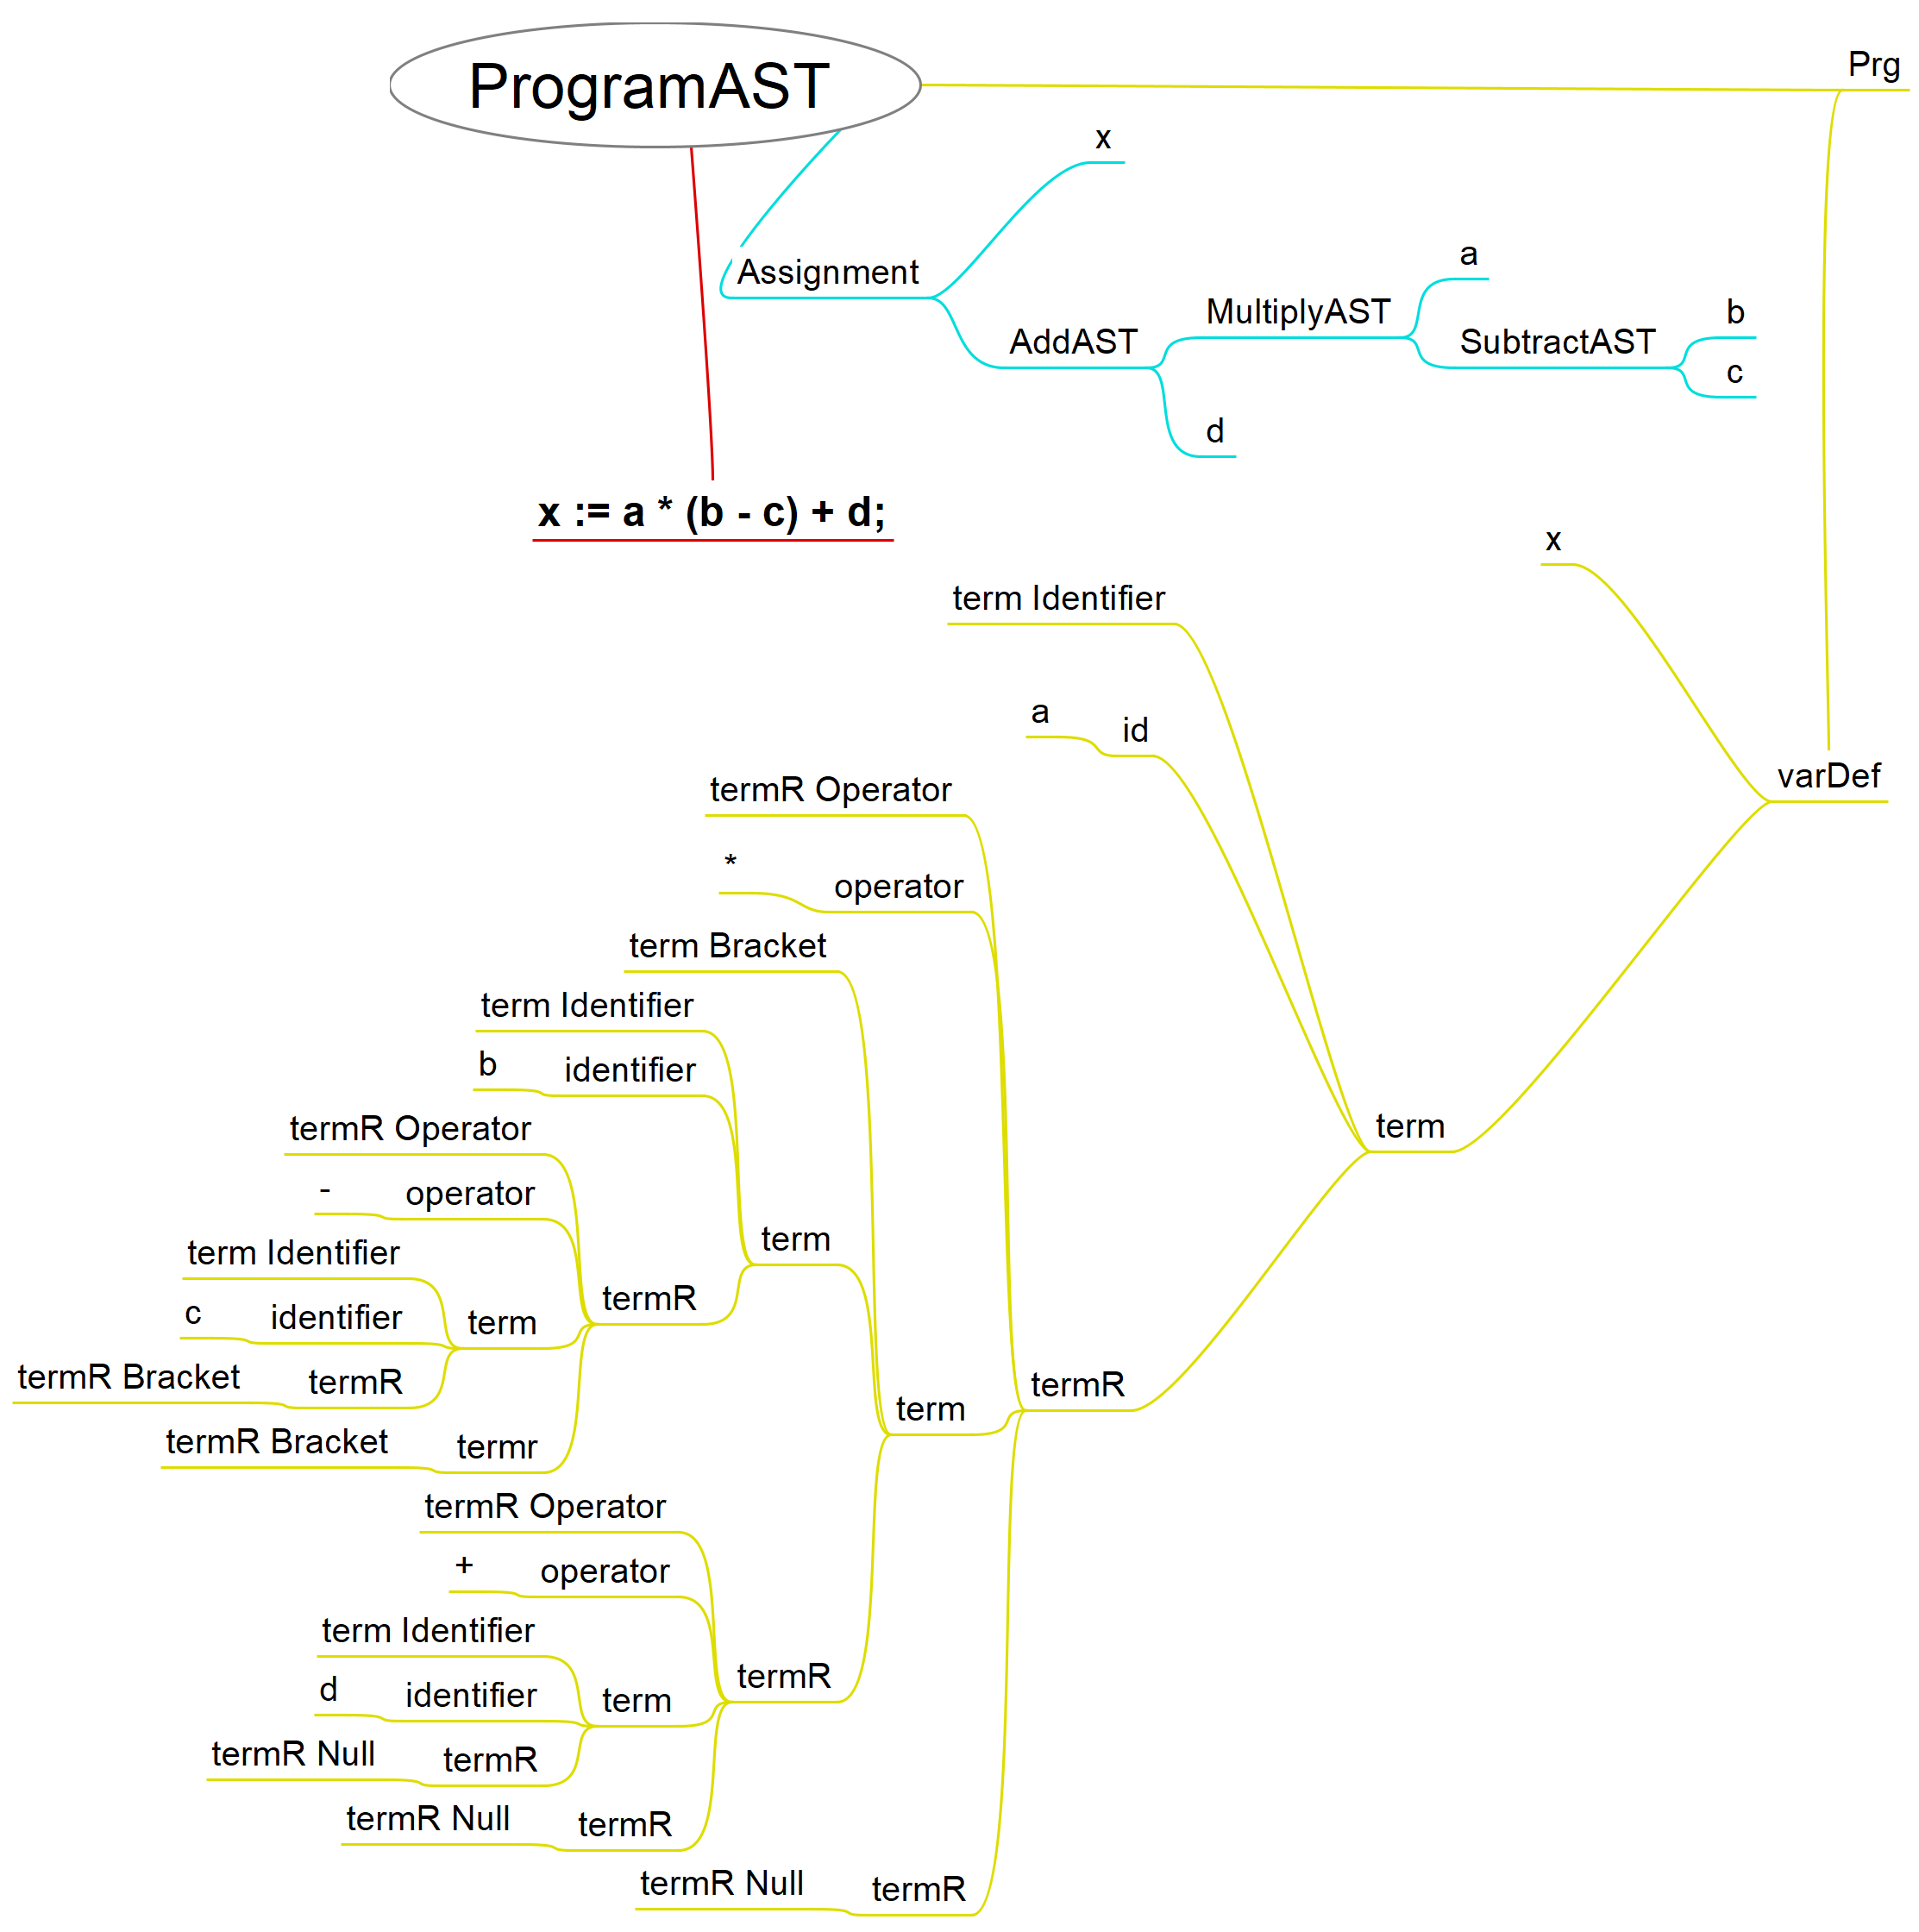
\includegraphics[width=1.0\linewidth]{images/parser-to-ast}
	\caption[Parser-Baum und AST]{Parser-Baum und AST anhand eines kleinen Beispiels}
	\label{fig:parseast}
\end{figure}

In diesem Unterkapitel wird ein kurzer Überblick über das Ziel des Parsers gegeben. Die Abbildung \ref{fig:parseast} zeigt anhand eines kleinen Codebeispiels, wie die zwei verschiedenen Strukturen aussehen, die während des Parsens erzeugt werden. Dabei wird das Programmcodebeispiel \mbox{\textbf{x := a * (b - c) + d;}} betrachtet. Der gelbe Pfad stellt die Struktur nach dem ersten Parsen des Codes da. Dabei ist \textbf{Prg} der Wurzelknoten und \textbf{varDef} dessen einziges Statement. Im blauen Pfad mit \textbf{ProgramAST} als Wurzelknoten ist der \textbf{Abstract Syntax Tree} abgebildet. Dieser wird im weiteren Verlauf vom Interpreter verwendet.

\subsection{Lexer}

Im Package \texttt{tokenizer} liegen einige Hilfsklassen, um das Parsen zu erleichtern. 
Hier sind die \texttt{Token} sehr wichtig. 
Der \texttt{Lexer} wandelt den übergebenen Programmcode mithilfe von Regular Expressions in Tokens um. Diese enthalten jeweils den zugehörigen Text, den Typ und die Position im Text, welche später beispielsweise zum Anzeigen von Exceptions benötigt wird. 
Der \texttt{Lexer} nutzt einen Pointer, der immer auf den aktuell betrachteten Token zeigt. Beim Start des Parsens ist dies der erste Token, also zum Beispiel das Erste Wort im Programmcode.

\subsubsection{Wichtige Funktionen}

Dieses Unterkapitel zeigt einen kurzen Überblick über die wichtigsten Funktionen, die im \texttt{Lexer} verwendet werden.
\newline
\textbf{lookahead()} gibt den aktuellen Token zurück. Mit einem int als Parameter kann auch auf einen Token zugegriffen werden, der erst später kommt.
\newline
\textbf{getNextToken()} gibt ebenfalls den aktuellen Token zurück. Allerdings verschiebt diese Funktion auch den TokenPointer um eins weiter.
\newline
\textbf{getNextTokenAndExpect(TokenExpression type)} macht das gleiche wie die vorherige Funktion. Allerdings wirft diese eine Exception, falls der aktuelle Token nicht den übergebenen Type besitzt.
\newline
\newline
Die Tokens selbst besitzen dann auch nochmal zwei Funktionen, die beim Parsen sehr oft verwendet werden.
\newline
\textbf{getType()} gibt den Type des aktuellen Tokens zurück, der dann beim Parsen dazu verwendet wird, um zu entscheiden, um was für ein Element es sich im jeweils folgenden Programmcode handelt. 
\newline
\textbf{getContent()} gibt den tatsächlichen Textinhalt des jeweiligen Tokens zurück.



\subsection{Parser-Baum}\label{subsection:parser}

\subsubsection{Überblick}

Beim Parser-Baum handelt es sich um eine direkte Umsetzung aus der gegebenen Sprachsyntax. 
Diese ist so gestaltet, dass keine Linksrekursionen auftreten können. 
Dabei enthält beispielsweise jeder Term einen TermR, welcher sozusagen einen Rest des Terms darstellt. 
Dieser kann entweder leer sein oder weitere Elemente enthalten. Dadurch ergibt sich für jeden Term eine Art verkettete Liste. 
\newline
\newline
In Abbildung \ref{fig:parseast} stellt der gelbe Ast den Parser-Baum dar, der entsteht, wenn das Programmcodebeispiel \mbox{\textbf{x := a * (b - c) + d;}} eingelesen wird. 
Der Wurzelknoten \texttt{Prg} beinhaltet eine ArrayList von Statements, die in diesem Beispiel nur ein Element und zwar eine VariablenDefinition enthält. 
Diese besteht wiederum aus einem Identifier \texttt{x}, der diese Variable darstellt und einem Term, der dieser Variable zugewiesen wird. 
Dieser Term ist der Identifier \texttt{a}, an dem ein TermR hängt, der wiederum einen Operator beinhaltet. Dies wird so lange fortgesetzt, bis das endgültige Ende des Terms erreicht wird.

\subsubsection{Umsetzung}

\begin{figure}[tbh]
	%\centering
	\hspace{-0.1\linewidth}
	%\fbox{}
	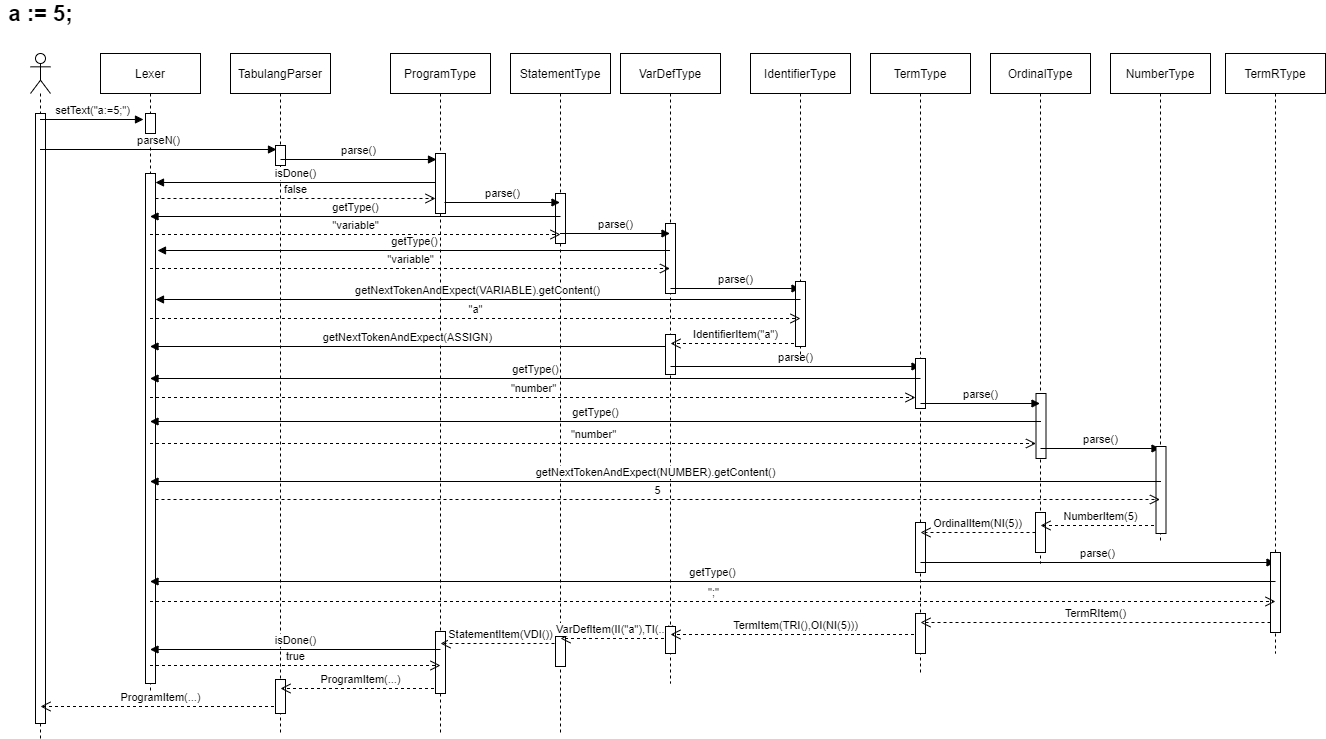
\includegraphics[width=1.2\linewidth]{images/sequenzdiagramm}
	\caption[Sequenzdiagramm Parser]{Sequenzdiagramm für die Erstellung des Parser-Baums}
	\label{fig:sequenzdiagramm}
\end{figure}

Alle Elemente im Parser-Baum erweitern die abstrakte Klasse \texttt{LanguageItemAbstract}. 
Diese beinhaltet einen \texttt{LanguageItemType}, der für die spätere Verarbeitung den Typ des jeweiligen Elements speichert, sowie eine \texttt{TextPosition}, die den Start- und Endpunkt enthält, welche für die Fehlerausgabe mit Positionsangabe benötigt wird.
Die jeweiligen Elemente selbst enthalten Fields für alle anderen Elemente, die es jeweils beinhalten kann. 
Welche das im Einzelnen sind, kann im Kapitel ''Syntax'' in der Sprachbeschreibung herausgefunden werden. Deshalb wird in dieser Dokumentation nicht weiter darauf eingegangen.
Alle dieser Elemente befinden sich im Package \texttt{items}. 
\newline
\newline
Das eigentliche Parsen geschieht mit Hilfe der \texttt{*Type}-Klassen.
Diese liegen im Package \texttt{items/types} und implementieren alle das \texttt{Parser}-Interface.
Das Interface enthält nur eine einzige Funktion \texttt{LanguageItemAbstract parse(Lexer l) throws ParseTimeException}. Diese Funktion beinhaltet in den Type-Klassen das Parsen des jeweiligen Elements anhand der Syntax und die Rückgabe eines Objekts für das Element.
\newline
\newline
Der Parsevorgang wird über die Funktion \texttt{parse()} in der Klasse \texttt{TabulangParser} im Package \texttt{parser} gestartet. Ab hier wird immer die \texttt{parse(l)}-Funktion der Instanz von der \texttt{*Type}-Klasse aufgerufen, deren Element im jeweiligen Kontext als nächstes erwartet wird. 
Dies kann zum einen daran entschieden werden, welche Typen laut der Syntax an der jeweiligen Stelle überhaupt zulässig sind und zum anderen daran, auf was für einen Token \texttt{Lexer} aktuell zeigt. 
Beim ersten Aufruf handelt es sich hier immer um ein \texttt{ProgramItem}, weshalb hier die Funktion \texttt{parse(l)} der Instanz der Klasse \texttt{ProgramType} aufgerufen wird.
Ein \texttt{ProgramItem} besteht wiederum aus einer Liste von Statements. Deshalb wird in einer Schleife so lange die Funktion \texttt{parse(l)} von \texttt{StatementType} aufgerufen, bis der \texttt{Lexer} als aktuelle TokenPosition das Ende des Programmcodes zurückgibt. Als Rückgabewert liefert diese dann jedes mal ein \texttt{StatementItem}, das an die Liste der Statements angehängt wird. In der aufgerufenen Parsefunktion wird Der TokenPointer immer entsprechend weitergeschoben, wenn ein Token verarbeitet wurde.

Bei dem aktuellen Token kann es sich beispielsweise um ein Schlüsselwort handeln, das zeigt, dass an dieser Stelle ein bestimmtes Element beginnt.
Zeigt \texttt{Lexer} zum Beispiel aktuell auf ein Token mit dem Inhalt ''return'' und an der aktuellen Stelle ist auch ein \texttt{ReturnStmntItem} erlaubt, so wird an dieser Stelle die Funktion \texttt{parse(l)} der Instanz der Klasse \texttt{ReturnStmntType} aufgerufen, welche, nachdem sie wiederum den kompletten Inhalt des Returnstatements verarbeitet hat, ein \texttt{ReturnStmntItem} zurückgibt.
\newline
\newline
In Abbildung \ref{fig:sequenzdiagramm} ist der Ablauf für die Erstellung des Parser-Baums an einem kleinen Beispiel aufgezeigt. Der Programmcode besteht in diesem Fall nur aus der einen Zeile mit dem Inhalt ''\textbf{a := 5;}''. Dabei handelt es sich um ein VarDef-Statement, das die Variable \textbf{a} erzeugt, falls diese nicht bereit existiert und dieser den Wert \textbf{5} zuweist.





\subsection{Abstract-Syntax-Tree (AST)}\label{subsection:ast}

